% !TEX root = ../OT4ML.tex

%%%%%%%%%%%%%%%%%%%%%%%%%%%%%%%%%%%%%%%%%%%%%%%%%%%%%%%%%%%%%%%%%%%%%%%%%%%
%%%%%%%%%%%%%%%%%%%%%%%%%%%%%%%%%%%%%%%%%%%%%%%%%%%%%%%%%%%%%%%%%%%%%%%%%%%
%%%%%%%%%%%%%%%%%%%%%%%%%%%%%%%%%%%%%%%%%%%%%%%%%%%%%%%%%%%%%%%%%%%%%%%%%%%
\section[Semi-discrete and W1]{Semi-discrete and $\Wass_1$}
\label{sec-semidiscr-w1}

This section focuses on two computationally useful degeneracies of the dual problem. Semi-discrete OT turns a continuous-to-discrete map into finite-dimensional geometry, while $\Wass_1$ replaces convex potentials by Lipschitz functions and flow fields. The material connects computational geometry~\cite{AurenhammerHA98,Merigot11,merigot2013comparison} with the Kantorovich--Rubinstein and Beckmann formulations~\cite{kantorovich1958space,Beckmann52}.

%%%%%%%%%%%%%%%%%%%%%%%%%%%%%%%%%%%%%%%%%%%%%%%%%%%%%%%%%%%%%%%%%%%%%%%%%%%
\subsection{Semi-dual}

The semi-dual eliminates one potential by an exact $c$-transform. It keeps concavity while removing explicit inequality constraints.

Write the dual problem~\eqref{eq-dual-generic} as
\eq{
	\usup{f,g \in \Cc(\Xx) \times \Cc(\Yy)} \Ee(f,g)
}
where $\Ee(f,g)$ is the dual objective, with value $-\infty$ when the feasibility constraint fails. One can optimize out $g$ exactly and obtain the following semi-dual problem
\eql{\label{eq-semi-dual}
	\usup{f \in \Cc(\Xx)} \tilde\Ee(f) \eqdef \Ee(f,f^c) = \usup{g} \Ee(f,g) =
	\int_\Xx f \d \al + \int_\Yy f^c \d \be.
}
Partial maximization of a concave problem preserves concavity, so $\tilde \Ee$ is still concave. The major advantage of the semi-dual is that it removes the explicit inequality constraint, which allows the use of simpler optimization algorithms.


%%%%%%%%%%%%%%%%%%%%%%%%%%%%%%%%%%%%%%%%%%%%%%%%%%%%%%%%%%%%%%%%%%%%%%%%%%%
\subsection{Semi-discrete}


The semi-discrete case is the setting where dual potentials become weights of Laguerre cells. This gives both geometry and algorithms for quantization and density fitting.

\paragraph{Discrete target and Laguerre cells.}

A case of particular interest is when $\be = \sum_j \b_j \de_{y_j}$ is discrete (of course the same construction applies if $\al$ is discrete by exchanging the role of $\al,\be$).
%
One can adapt the definition of the $\bar c$ transform~\eqref{eq-c-transform} to this setting by restricting the minimization to the support $(y_j)_j$ of $\be$,
\eql{\label{eq-disc-c-transfo}
	\foralls \gD \in \RR^m, \;
	\foralls x \in \Xx, \quad
	\gD^{\bar \c}(x) \eqdef \umin{j \in \range{m}} \c(x,y_j) - \gD_j.
}
This transform maps a vector $\gD$ to a continuous function $\gD^{\bar \c} \in \Cc(\Xx)$ under the same regularity assumptions on $c$ as in the continuous setting.
%
Note that this definition coincides with~\eqref{eq-c-transform} when the target space $\Y$ is restricted to the support of $\be$.

Crucially, using the discrete $\bar c$-transform, when $\be$ is a discrete measure, yields a finite-dimensional optimization,
\eql{\label{eq-semi-dual-discr}
	\MK_\c(\al,\be) =
		\umax{\gD \in \RR^m}
			\Ee(\gD) \eqdef
			\int_\X \gD^{\bar \c}(x) \d\al(x) + \sum_j \gD_j \b_j.
}

The Laguerre cells associated to the dual weights $\gD$
\eql{\label{eq-laguerre-cells}
	\Laguerre_{j}(\gD) \eqdef \enscond{x \in \X}{ \foralls j' \neq j, \c(x,y_j) - \gD_j \leq \c(x,y_{j'}) - \gD_{j'} }
}
cover $\X$. After arbitrary tie-breaking on common boundaries, they induce a disjoint partition; when $\gD$ is constant, this partition is the ordinary Voronoi diagram.
%
For quadratic costs, varying the dual weights moves the walls between adjacent cells while keeping them parallel; this is the geometric mechanism by which the cell masses are adjusted.
%
\begin{figure}[H]
\centering
\begin{tabular}{@{}ccc@{}}
\small zero weights &
\small intermediate weights &
\small balanced cells \\[-.15em]
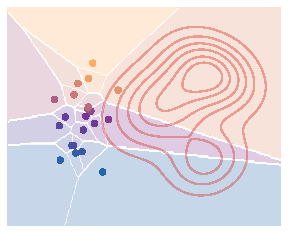
\includegraphics[width=.30\linewidth]{figures/semidiscrete-laguerre-cells/voronoi.pdf} &

\includegraphics[width=.30\linewidth]{figures/semidiscrete-laguerre-cells/weighted.pdf} &

\includegraphics[width=.30\linewidth]{figures/semidiscrete-laguerre-cells/balanced.pdf}
\end{tabular}
\caption{Laguerre cells for semi-discrete quadratic transport.  The red contours show a continuous source density $\al$ given by a three-component Gaussian mixture on the right.  The twenty-one colored circular sites are the atoms of the discrete target $\be$ sampled from a compact Gaussian cloud on the left; each site color matches its Laguerre cell.  Starting from ordinary Voronoi cells, semi-dual weight updates deform the cells so that the $\al$-mass captured by each cell approaches the prescribed target mass.}
\label{fig:semidiscrete-laguerre-cells}
\end{figure}

\paragraph{Mass balance.}

This allows one to conveniently rewrite the semi-dual energy as
\eql{\label{eq-semi-disc-energy}
	\Ee(\gD) = \sum_{j=1}^m \int_{\Laguerre_{j}(\gD)} \pa{ c(x,y_j) - \gD_j } \d\al(x) + \dotp{\gD}{\b}.
}
The following proposition provides a formula for the gradient of this concave function.

\begin{prop}[Gradient of the semi-discrete dual]
If $\al$ gives zero mass to the Laguerre cell boundaries, then $\Ee$ is differentiable at $\gD$ and
\eq{
	\foralls j \in \range{m}, \quad
	\nabla\Ee(\gD)_j = \b_j - \int_{\Laguerre_{j}(\gD)} \d\al.
}
\end{prop}
\begin{proof}
	For $\al$-almost every $x$, the minimizing index in $\min_j c(x,y_j)-\gD_j$ is unique. If this index is $j(x)$, then the directional derivative in a direction $h\in\RR^m$ is
	\[
		\left.\frac{\d}{\d t}\right|_{t=0}
		\min_j \bigl(c(x,y_j)-(\gD_j+t h_j)\bigr)
		=
		-h_{j(x)}.
	\]
	Dominated convergence gives
	\[
		\d\Ee(\gD)[h]
		=
		-\sum_j h_j\int_{\Laguerre_j(\gD)}\d\al
		+\sum_j h_j\b_j,
	\]
	which is the announced gradient formula.
\end{proof}

The first-order optimality condition shows that solving the dual semi-discrete problem amounts to choosing the weights $\gD$ so that $\int_{\Laguerre_{j}(\gD)} \d\al = \b_j$, i.e. each cell captures the prescribed amount of mass. In this case, the optimal transport $T$ with $T_\sharp \al=\be$ is piecewise constant and maps $x \in \Laguerre_{j}(\gD)$ to $y_j$; for the quadratic cost, uniqueness follows from Brenier's theorem when $\al$ has a density.

In the special case $c(x,y)=\norm{x-y}^2$, the Laguerre decomposition is also called a power diagram. Its cells are polyhedral, and can be computed efficiently using computational geometry algorithms~\cite{aurenhammer1987power,AurenhammerHA98,Merigot11}. One classical construction lifts the sites to points $(y_j,\norm{y_j}^2-\gD_j)\in\RR^{d+1}$ and obtains the power diagram by projecting the lower envelope of their convex hull. In dimensions two and three, Chan's output-sensitive convex-hull algorithm~\cite{chan1996optimal} has complexity $O(m\log Q)$ for $m$ sites and $Q$ hull vertices.

\paragraph{Stochastic optimization.}

The semi-discrete formulation~\eqref{eq-semi-disc-energy} is useful because the objective is an expectation with respect to $\al$,
\eql{\label{eq-semi-disc-energy-entropy}
	\Ee(\gD)
	=
	\int_\X E(\gD,x)\d\al(x)
	=
	\EE_X(E(\gD,X)),
	\qquad
	E(\gD,x)\eqdef \gD^{\bar c}(x)+\dotp{\gD}{\b}.
}
Here $X\sim\al$. Away from cell boundaries, the stochastic gradient of the integrand is
\[
	\nabla_{\gD}E(\gD,x)
	=
	\left(\b_j-\ones_{\Laguerre_j(\gD)}(x)\right)_{j=1}^m,
\]
which is an unbiased estimator of $\nabla\Ee(\gD)$ when cell boundaries have $\al$-measure zero. One can therefore maximize~\eqref{eq-semi-disc-energy} without first discretizing $\al$: the measure is used as a black box from which independent samples are drawn, a natural setup in high-dimensional statistics and machine learning.

Starting from $\gD^{(0)}=0$, stochastic gradient ascent draws $x_\ell\sim\al$ and performs
\eql{\label{eq-sgd}
	\gD^{(\ell+1)}
	\eqdef
	\gD^{(\ell)}+\tau_\ell\nabla_{\gD}E(\gD^{(\ell)},x_\ell).
}
The step size must decay so that the sampling noise averages out. A typical schedule is
\eql{\label{eq-step-size-sgd}
	\tau_\ell\eqdef \frac{\tau_0}{1+\ell/\ell_0},
}
where $\ell_0$ is a warmup scale. Under standard stochastic-approximation assumptions, one obtains the usual sublinear rate
\[
	\Ee(\gD^\star)-\EE\big(\Ee(\gD^{(\ell)})\big)
	=
	O(\ell^{-1/2}),
\]
where $\gD^\star$ is a maximizer and the expectation is over the i.i.d. samples. This stochastic viewpoint is one of the main algorithmic advantages of the semi-discrete formulation~\cite{Merigot11,genevay2016stochastic}.


%%%%%%%%%%%%%%%%%%%%%%%%%%%%%%%%%%%%%%%%%%%%%%%%%%%%%%%%%%%%%%%%%%%%%%%%%%%
\subsection{Optimal Quantization}
\label{sec-optimal-quantization}

Optimal quantization asks for the best discrete approximation of a measure by $m$ codepoints. It is the geometric core of vector quantization, compression and $k$-means clustering.

The optimal quantization problem for a measure $\al$ is
\eql{\label{eq-optimal-quantization}
	\Qq_m(\al)
	\eqdef
	\umin{Y=(y_j)_{j=1}^m,\ \b\in\simplex_m}
	\Wass_p\left(\al,\sum_{j=1}^m \b_j\de_{y_j}\right).
}
This problem is classical in approximation theory and information theory~\cite{graf2000foundationsquantization,Lloyd82}. The OT formulation emphasizes that one optimizes both the support locations $Y$ and, unless prescribed, the masses $\b$.

\begin{prop}[Quantization rate and curse of dimensionality]\label{prop-quantization-rate}
	Let $\Omega\subset\RR^d$ be a bounded Lipschitz domain and assume $\al=\rho\,\d x$ on $\Omega$, with $0<\rho_-\leq\rho\leq\rho_+<+\infty$. Then, for fixed $p\geq1$, there exist constants $0<c\leq C<+\infty$ such that
	\[
		c\,m^{-1/d}
		\leq
		\Qq_m(\al)
		\leq
		C\,m^{-1/d}.
	\]
\end{prop}
\begin{proof}
	For the upper bound, partition $\Omega$ into $m$ cells of diameter at most $Cm^{-1/d}$, up to boundary effects, and put one codepoint in each non-empty cell. Sending each point to the codepoint in its cell gives a transport distance bounded by $Cm^{-1/d}$.

	For the lower bound, fix any set $Y$ of $m$ codepoints and write $d_Y(x)=\min_j\norm{x-y_j}$. Since the density is bounded above, the mass of the $t$-neighborhood of $Y$ is at most $Cmt^d$. Choosing $t_0\simeq m^{-1/d}$ small enough gives $\al(\{d_Y>t\})\geq c$ for $0<t<t_0$. Hence
	\[
		\int d_Y(x)^p\d\al(x)
		=
		\int_0^{+\infty} p t^{p-1}\al(\{d_Y>t\})\d t
		\geq
		c t_0^p
		\simeq
		c m^{-p/d}.
	\]
	Taking the $p$-th root and minimizing over $Y$ proves the lower bound.
\end{proof}

This deterministic rate mirrors the empirical OT sample-complexity rate: both are governed by the spacing $m^{-1/d}$ of points in dimension $d$. Quantization is best-case and deterministic, while empirical OT is random, but both display the same curse of dimensionality.
For fixed codepoints $Y$, the problem is convex with respect to the weights $\b$. The dependence on $Y$ is non-convex and is generally computationally hard. The one-dimensional case is substantially simpler: monotonicity fixes the ordering of the cells, reducing the problem to interval endpoints and centroids; for the uniform law with the quadratic cost, the optimal centroids are equally spaced.

\begin{prop}[Free masses give Voronoi cells]\label{prop-free-masses-voronoi}
	For the cost $c(x,y)=d(x,y)^p$, fix distinct codepoints $Y=(y_j)_{j=1}^m$. Duplicate codepoints can be merged beforehand. Minimizing over the weights $\b\in\simplex_m$ gives
	\[
		\min_{\b\in\simplex_m}
		\Wass_p^p\left(\al,\sum_j \b_j\de_{y_j}\right)
		=
		\int_\X \min_{1\leq j\leq m} c(x,y_j)\d\al(x).
	\]
	An optimal coupling is induced by sending each $x$ to a nearest codepoint. The corresponding cells are the Voronoi cells
	\[
		\VV_j(Y)
		\eqdef
		\enscond{x}{\foralls j',\ c(x,y_j)\leq c(x,y_{j'})},
	\]
	up to arbitrary tie-breaking on common boundaries.
\end{prop}
\begin{proof}
	For any coupling between $\al$ and a measure supported on $Y$, the conditional destination of a point $x$ belongs to $Y$, hence its conditional cost is at least $\min_j c(x,y_j)$. Integrating gives the lower bound. Conversely, choose a measurable nearest-codepoint map $T_Y(x)\in\argmin_j c(x,y_j)$, breaking ties measurably, and set $\b_j=\al(T_Y^{-1}(y_j))$. Then $(T_Y)_\sharp\al=\sum_j \b_j\de_{y_j}$ and the induced transport reaches the displayed lower bound.
\end{proof}

Consequently, the quantization energy can be written in the nearest-centroid form
\[
	\Qq_m(\al)^p
	=
	\min_Y \Ff(Y),
	\qquad
	\Ff(Y)
	\eqdef
	\int_\X \min_{1\leq j\leq m} c(x,y_j)\d\al(x).
\]
At a differentiability point of this energy, each local minimizer satisfies the centroid condition
\[
	y_j
	\in
	\uargmin{y}
	\int_{\VV_j(Y)} c(x,y)\d\al(x).
\]
For the squared Euclidean cost, this becomes the fixed-point equation
\[
	y_j
	=
	\frac{\int_{\VV_j(Y)} x\d\al(x)}
	{\int_{\VV_j(Y)} \d\al}.
\]
Lloyd's algorithm, also known as the $k$-means algorithm, iterates this fixed point: assign points to nearest sites, then replace each site by the centroid of its cell~\cite{Lloyd82}. With standard tie-breaking, the objective decreases at each step. Since the problem is non-convex in $Y$, the iterates generally converge only to a local minimum. Good seeding matters; for the squared Euclidean objective, $k$-means++ gives a logarithmic approximation guarantee in expectation~\cite{ArthurVassilvitskii2007}.

\begin{figure}[H]
\centering
\begin{tabular}{@{}ccc@{}}
\small initialization &
\small after $6$ iterations &
\small after $36$ iterations \\[-.15em]

\includegraphics[width=.30\linewidth]{figures/semidiscrete-lloyd-quantization/initial.pdf} &
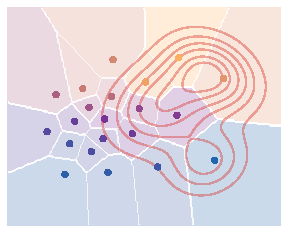
\includegraphics[width=.30\linewidth]{figures/semidiscrete-lloyd-quantization/iter6.pdf} &
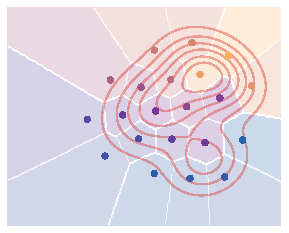
\includegraphics[width=.30\linewidth]{figures/semidiscrete-lloyd-quantization/iter36.pdf}
\end{tabular}
\caption{Lloyd quantization for the same continuous density and twenty-one initial sites as Figure~\ref{fig:semidiscrete-laguerre-cells}.  The red contours show the density $\al$, while the colored disks are the current codepoints and have the same colors as their Voronoi cells.  The iterations move the initially left-located sites toward the high-density region and reshape the cells according to centroidal Voronoi geometry.}
\label{fig:semidiscrete-lloyd-quantization}
\end{figure}


%%%%%%%%%%%%%%%%%%%%%%%%%%%%%%%%%%%%%%%%%%%%%%%%%%%%%%%%%%%%%%%%%%%%%%%%%%%
\subsection[W1]{Wasserstein-1 norm}
\label{sec-W1}

The $\Wass_1$ distance has an especially transparent dual: the admissible potentials are exactly $1$-Lipschitz test functions. This makes $\Wass_1$ the meeting point between transport, PDE formulations and weak norms on signed measures.

\paragraph{$c$-transform for $\Wass_1$.}

Assume that $d$ is a distance on $\X=\Y$ and take the ground cost $c(x,y)=d(x,y)$. We denote the Lipschitz constant of $f\in\Cc(\X)$ by
\eql{\label{eq-lip-constant}
	\Lip(f)
	\eqdef
	\sup\enscond{\frac{|f(x)-f(y)|}{d(x,y)}}{x\neq y}.
}

\begin{prop}[$c$-transforms and $1$-Lipschitz functions]\label{prop-w1-c-transform-lipschitz}
	Suppose $\X=\Y$ and $c(x,y)=d(x,y)$. Then there exists $g$ such that $f=g^c$ if and only if $\Lip(f)\leq1$. Furthermore, if $\Lip(f)\leq1$, then $f^c=-f$.
\end{prop}
\begin{proof}
	First suppose $f=g^c$ for some $g$. For $x,y\in\X$,
	\[
		|f(x)-f(y)|
		=
		\left|\inf_z[d(x,z)-g(z)]-\inf_z[d(y,z)-g(z)]\right|
		\leq
		\sup_z |d(x,z)-d(y,z)|
		\leq d(x,y),
	\]
	where the last inequality is the reverse triangle inequality. Thus $\Lip(f)\leq1$.

	If $\Lip(f)\leq1$, then $f(x)\leq f(y)+d(x,y)$, so $d(x,y)-f(x)\geq -f(y)$ for all $x$ and hence $f^c(y)\geq -f(y)$. Taking $x=y$ gives $f^c(y)\leq -f(y)$. Therefore $f^c=-f$. Applying the same property to $-f$ gives $(-f)^c=f$, so every $1$-Lipschitz function is $c$-concave.
\end{proof}

Using the alternating $c$-transform scheme~\eqref{eq-iter-c-trans}, one can replace the dual pair by $(f,-f)$ with $\Lip(f)\leq1$. The Kantorovich dual therefore becomes the Kantorovich--Rubinstein formula
\eql{\label{eq-w1-metric}
	\Wass_1(\al,\be)
	=
	\umax{f}
	\enscond{\int_\X f\d(\al-\be)}{\Lip(f)\leq1}.
}
This expression depends only on the signed measure $\al-\be$. It therefore extends to finite signed measures of total mass zero and defines the Kantorovich--Rubinstein norm on that space~\cite{kantorovich1958space}.

For a discrete signed measure $\al-\be=\sum_k r_k\de_{z_k}$ with $\sum_k r_k=0$,~\eqref{eq-w1-metric} becomes the finite-dimensional linear program
\eql{\label{eq-w1-discr}
	\Wass_1(\al,\be)
	=
	\umax{(f_k)_k}
	\enscond{\sum_k f_k r_k}{\foralls k,\ell,\ |f_k-f_\ell|\leq d(z_k,z_\ell)}.
}
This linear program can be solved by generic interior-point or first-order methods; structured graph versions admit the flow formulations described below.
When $d(x,y)=|x-y|$ on $\RR$, ordering the support points $z_1\leq z_2\leq\cdots$ reduces the constraints to neighboring pairs,
\[
	\Wass_1(\al,\be)
	=
	\umax{(f_k)_k}
	\enscond{\sum_k f_k r_k}{\foralls k,\ |f_{k+1}-f_k|\leq z_{k+1}-z_k}.
\]
In one dimension this is equivalent to the closed-form cumulative formula introduced earlier.

\paragraph{$\Wass_1$ on Euclidean spaces.}

In the special case of Euclidean spaces $\X=\Y=\RR^\dim$, using $\c(x,y) = \norm{x-y}$, the global Lipschitz constraint in the Kantorovich--Rubinstein formula can be made local as a uniform bound on the gradient of $f$,
\eql{\label{eq-w1-cont}
	\Wass_1(\al,\be) =
	\usup{f} \enscond{ \int_{\RR^\dim} \f (\d\al-\d\be) }{ \norm{\nabla \f}_\infty \leq 1 }.
}
Here the constraint $\norm{\nabla \f}_\infty \leq 1$ signifies that the norm of the gradient of $\f$ at any point $x$ is upper bounded by $1$, $\norm{\nabla \f(x)}_2 \leq 1$ for any $x$.

Considering the dual problem to~\eqref{eq-w1-cont}, denoting $\xi \eqdef \al-\be$, and using the equivalent form
\eq{
	-\iota_{\norm{\cdot}_{\RR^d} \leq 1}(u) = \uinf{v} \dotp{u}{v} + \norm{v}_{\RR^d},
}
one has a maximization on flow vector fields $\flow :  \RR^d \rightarrow \RR^d$
\begin{align*}
	\Wass_1(\al,\be) &=
	\usup{f} \uinf{\flow(x) \in \RR^d} \int_{\RR^\dim} \f \d\xi + \int \dotp{\nabla f(x)}{\flow(x)} \d x + \int \norm{\flow(x)}_{\RR^d} \d x \\
	&=
	\uinf{\flow(x) \in \RR^d} \int \norm{\flow(x)} \d x
		+ \usup{f} \int f(x) ( \d \xi - \diverg(\flow) \d x)
\end{align*}
one obtains an optimization problem under a fixed divergence constraint
\eql{\label{eq-w1-cont-div}
	\Wass_1(\al,\be) =
	\uinf{\flow} \enscond{ \int_{\RR^\dim} \norm{\flow(x)}_{\RR^d} \d x }{  \diverg(\flow)=\al-\be },
}
which is often called the Beckmann formulation~\cite{Beckmann52}.
%
Here the vectorial function $\flow(x) \in \RR^\dim$ can be interpreted as a flow field, describing locally the movement of mass. Outside the support of the two input measures, $\diverg(\flow)=0$, which is the conservation of mass constraint.
%
Once properly discretized using finite elements, Problems~\eqref{eq-w1-cont} and~\eqref{eq-w1-cont-div} become a nonsmooth convex optimization problem.

The previous formulations~\eqref{eq-w1-cont} and~\eqref{eq-w1-cont-div} of $\Wass_1$ can be generalized to the setting where $\X$ is a Riemannian manifold, i.e. $\c(x,y)=\dist(x,y)$ where $\dist$ is the associated geodesic distance (and then for smooth manifolds, the gradient and divergence should be understood as differential operators on manifolds).

\begin{prop}[$\Wass_1$ and Beckmann flow on a graph]\label{prop-graph-w1-beckmann}
	Let $G=(V,E)$ be a connected finite graph with positive edge lengths $(\ell_e)_{e\in E}$. The graph geodesic distance is
	\[
		d_G(i,j)=\min_{\gamma:i\leadsto j}\sum_{e\in\gamma}\ell_e.
	\]
	For two probability vectors $\a,\b$ on $V$, set $r=\a-\b$ and orient each edge $e=(i,j)$. If
	\[
		(\nabla_G f)_e=f_j-f_i,\qquad
		\operatorname{div}_G=-\nabla_G^*
	\]
	are the finite-difference gradient and its negative adjoint, then a positive flow on the oriented edge $i\to j$ has positive divergence at $i$ and negative divergence at $j$. With this convention,
	\[
		\Wass_{1,G}(\a,\b)
		=
		\max_f \enscond{\sum_{i\in V} f_i r_i}{|f_i-f_j|\leq \ell_e\quad\forall e=(i,j)}
		=
		\min_m \enscond{\sum_{e\in E}\ell_e |m_e|}{\operatorname{div}_G m=r}.
	\]
	The vector $m_e$ is an oriented edge flow, and the constraint $\operatorname{div}_G m=r$ is conservation of mass at each vertex.
\end{prop}

\begin{proof}
	The edge constraint $|f_i-f_j|\leq\ell_e$ implies, by summing along paths, that $|f_i-f_j|\leq d_G(i,j)$ for all vertices. Conversely, any $1$-Lipschitz function for $d_G$ satisfies the edge constraints because each edge is a path of length $\ell_e$. The first equality is therefore the Kantorovich--Rubinstein formula on the metric space $(V,d_G)$.

	For the second equality, write the graph Beckmann problem and dualize its equality constraint with a potential $f$:
	\[
		\inf_m \sum_e\ell_e|m_e|
		+\sup_f \sum_i f_i(r_i-(\operatorname{div}_G m)_i).
	\]
	Using $\operatorname{div}_G=-\nabla_G^*$, the coupling term is $\sum_e m_e(\nabla_G f)_e$. The minimization over each scalar flow $m_e$ is finite exactly when $|(\nabla_G f)_e|\leq\ell_e$, and is then equal to zero. The dual problem is therefore precisely the graph Lipschitz dual above. Strong duality holds because this is a finite-dimensional linear program with a non-empty feasible set: connectedness and $\sum_i r_i=0$ allow the signed surplus to be routed along paths. This proves the graph Beckmann formula.
\end{proof}

\begin{figure}[H]
\centering
\begin{tabular}{cc}
\small signed masses on $G$ &
\small optimal edge flow \\[-.15em]

\includegraphics[width=.40\linewidth]{figures/w1-graph-transport-flow/masses.pdf} &

\includegraphics[width=.40\linewidth]{figures/w1-graph-transport-flow/flow.pdf}
\end{tabular}
\caption{Graph Beckmann formulation of $\Wass_1$ on a Delaunay graph $G=(V,E)$ with $36$ vertices.  Red and blue disks encode the positive and negative parts of $r=\alpha-\beta$, localized on five vertices each.  The violet arrows display the optimal signed edge flow $m$: orientation gives the sign, width is proportional to $\sqrt{|m_e|}$, and the flow satisfies the conservation constraint $\operatorname{div}_G m=r$.}
\label{fig:w1-graph-transport-flow}
\end{figure}

This graph formulation is the transshipment version of $\Wass_1$. It is the natural discrete analogue of~\eqref{eq-w1-cont-div}: gradients are edge differences, divergences are incidence-matrix balances, and geodesic distance is the shortest-path length. It can be solved by min-cost flow methods on sparse graphs, and entropic or KL-projection variants lead to flow-Sinkhorn algorithms for graph $\Wass_1$~\cite{Beckmann52,peyre2026robust}.
